\section{Design}

\subsection{Database Design}
The project should have a database to store data. 
The data are batch's see figure \ref{figure:eer_diagram_batch} and users see 
figure \ref{figure:eer_diagram_users}. The data is useful for making a complete
system for Refslevbæk Bryghus A/S, then they can make sure to have the control
over who can use the system and have a report over what the machine is producing.

\myworries{
    The group are going to need a database or multiple to hold information on the 
    users and batch's you can see the figure \ref{figure:eer_diagram_batch} and 
    \ref{figure:eer_diagram_users} for reference.
    The multiple database part depends how much the system is in need for splitting up. 
    In the groups scope, it would make sense too keep it in one database, because 
    there are not many writes to the database.
}

\subsubsection{batch's}%
\label{ssub:batch_s}
The Batch's database is used in the system to keep track of batch's.
For example if a person would like to know what happened then the beer got produced,
like what temperature was it then the temperature was highest, Did that ruin it.
How much was defect.

\begin{figure}[ht]
\centering 
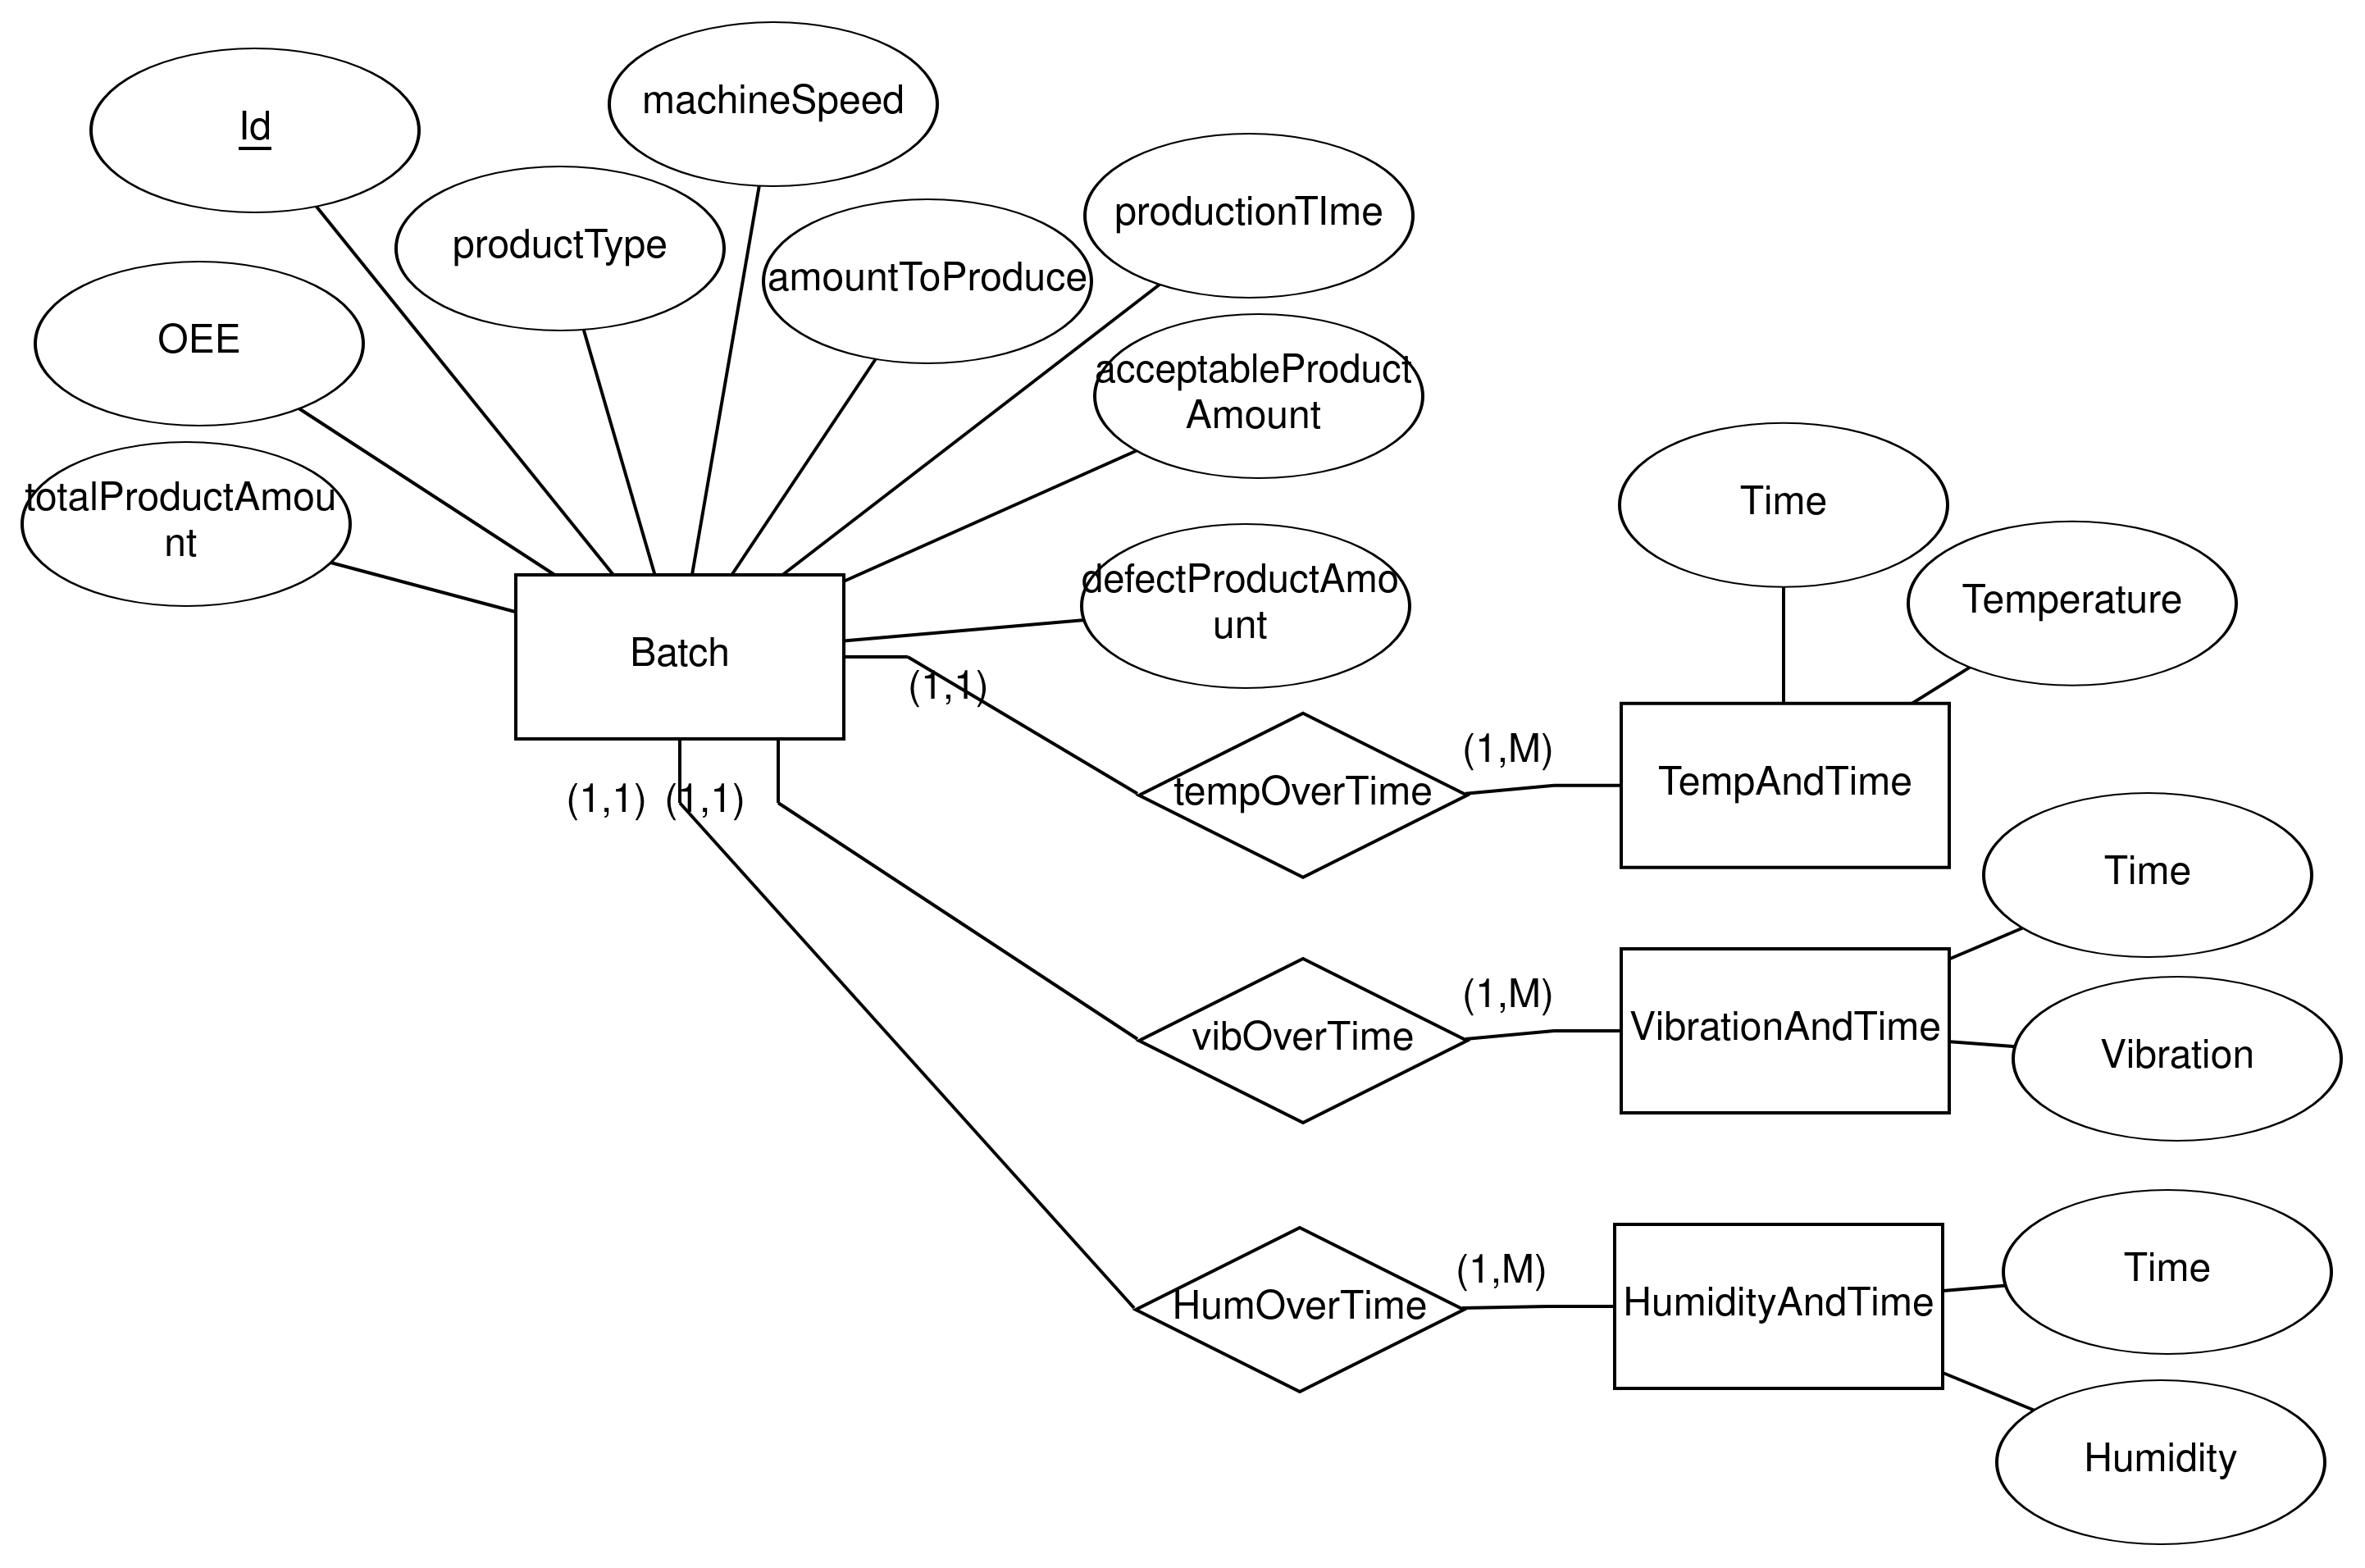
\includegraphics[width=0.8\linewidth]{images/eer_diagrams/database_EER_batch.png}
\caption{IR diagram for batch} 
\label{figure:eer_diagram_batch}
\end{figure}

\subsubsection{users}%
\label{ssub:users}


\myworries{Not sure if we should have user database for the system
    depends if the system need a authorisation? Like the web page(client) talk 
    to the server should it be all users or just the once that is registered in
    the system, with passwords?}

The user database is used in the system to keep track of users who are allow to
login. For example if a person want to start a beer production, then the user 
need to login. The user then hit the \textbf{API} with a login request. 
The \textbf{API} queris the database. The database then look up the query and 
then send a respone back with the information, if there is none it will send a
empty respone else it just send the information back to the \textbf{API}.
\begin{figure}[ht]
\centering 
\includegraphics[width=0.55\linewidth]{images/eer_diagrams/users.png}
\caption{EER diagram for users} 
\label{figure:eer_diagram_users}
\end{figure}
